%% !TEX encoding = UTF-8 Unicode
%
%% !TEX root = ObiStein.tex
%
%%---------------------
%\title{Ireneo Peral: mi hermano mayor}
%\author{Juan Carlos Peral}
%%---------------------
%
%%---------------------
%\contact{Juan Carlos Peral, Departamento de Matemáticas, Universidad del País Vasco}
%{juancarlos.peral@ehu.es}{}
%%---------------------
%
%%---------------------
%\makesemititle
%%---------------------


\subsection{Ireneo Peral: mi hermano mayor}

\begin{center}\large
\textbf{Juan Carlos Peral}\\[1em] 
Universidad del Pa\'{\i}s Vasco/Euskal Herriko Unibertsitatea
{\color{azulsema}\rule{.5\linewidth}{1pt}}
\end{center}

\vskip 5mm



En estas l\'ineas me referir\' e a mi hermano Ireneo, que nos  dej\'o  de forma prematura el d\'ia 16 de febrero de 2021.
No entrar\'e en su   trabajo matem\'atico porque otros, con mayor conocimiento del mismo, ya lo glosan en estas p\'aginas.



 Han pasado unos meses desde el fallecimiento de Ireneo, mi querido hermano mayor, y en este tiempo hay dos ideas que vuelven una y otra vez a mi mente y creo que reflejan bien mis sensaciones tras su inesperada muerte.
 
La primera se puede resumir con este verso de un poeta de la generaci\'on del 27:

\begin{quote}
\textit{Cuando yo vine al mundo, ya estaba todo hecho.} (Luis Felipe Vivanco)
\end{quote}

Para m\'i, su significado describe muy bien mis sentimientos sobre el papel tutelar y el profundo sentido familiar  que mi hermano tuvo siempre y que yo experiment\'e desde la infancia. Ireneo, Ito como le llam\'abamos nosotros, era cuatro a\~nos mayor que yo y era el que en los lejanos tiempos de nuestra infancia y adolescencia, primero en Madrid,  donde nacimos \'el, nuestra hermana Mar\'ia del Carmen y yo,  y luego en Bercimuelle (Salamanca), donde nacieron los dos  peque\~nos, Juli\'an y Germ\'an, era, como dec\'{\i}a,  el hermano mayor, el protector que cuidaba de m\'i en la escuela de Bercimuelle si alg\'un chico osaba meterse conmigo. M\'as de uno se llev\'o un buen pescoz\'on por intentarlo.

Compart\'{\i}amos habitaci\'on y muchas veces desde su cama en voz alta hac\'{\i}a como si fuese un locutor de radio y  relataba sus cr\'onicas para que yo las escuchase, absolutamente embelesado,  desde la m\'{\i}a. Pod\'{\i}a tratarse de las victorias de su equipo de f\'utbol favorito, como es bien sabido el Real Madrid, o de relatos de la actualidad diaria o referencias a noticias importantes de aquellos tiempos,  como el asesinato de Kennedy.
Tras estos a\~nos, en Bercimuelle, Ireneo curs\'o sus estudios preuniversitarios y el primer curso de universidad en Salamanca. Se alojaba en una pensi\'on de la calle San Justo. Curiosamente la misma calle en la que vivieron unos a\~nos nuestros abuelos paternos y nuestro padre, Ireneo, mientras comenzaba, tambi\'en \'el, sus estudios de Exactas, como se dec\'{\i}a entonces para referirse  a las Matem\'aticas.

Durante ese curso en Salamanca  sucedi\'o algo fundamental en su vida: conoci\'o a Magdalena, que era compa\~nera de clase. 
A\~nos  despu\'es se casar\'{\i}an frente al bellis\'{\i}mo  retablo de Nicol\'as Florentino en la catedral rom\'anica de Salamanca,  m\'as conocida como la Catedral Vieja. 
Tambi\'en en  ese curso en Salamanca   decidi\'o que estudiar\'{\i}a matem\'aticas.

\begin{figure}%[h]
\begin{center}
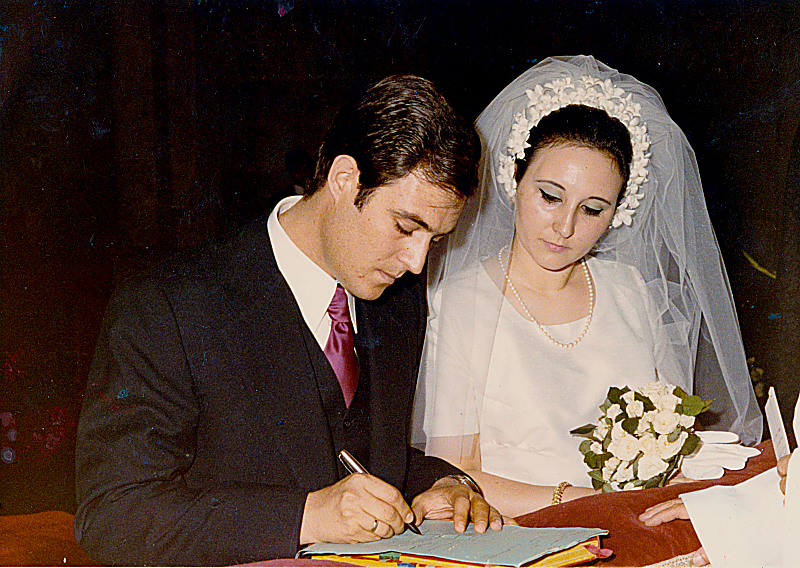
\includegraphics[width=0.9\linewidth]{IP_foto_boda.jpg}
\caption{Ireneo y Magdalena.}
\end{center}
\end{figure}


Las matem\'aticas eran algo natural en nuestra casa ya que nuestro padre, como licenciado en Matem\'aticas, ten\'{\i}a  ejemplares del an\'alisis de Goursat, de la geometr\'{\i}a proyectiva de Enriques o de las gruesas  tablas de logaritmos de Schron y otros  muchos textos de la \'epoca, libros  que a\'un conservamos.
De vez en cuando nuestro padre nos daba clase en un viejo encerado negro mientras nuestra madre, Mar\'ia del Carmen, se ocupaba de la casa.

Esa elecci\'on  de las Matem\'aticas  hecha por mi hermano me acab\'o de decidir a m\'i tambi\'en por la misma disciplina.
Es decir, mi hermano ha supuesto no solo una especie de manto protector en mi infancia, sino tambi\'en alguien que iba sirviendo de gu\'{\i}a y abriendo camino en diferentes aspectos.

Creo que esto explica esa sensaci\'on que me trasmite el verso que citaba al principio, y que ahora transcribo de nuevo, \textit{cuando yo vine al mundo, ya estaba todo hecho}, cuando pienso en mi hermano Ireneo.

Pasados estos a\~nos en Bercimuelle la familia volvi\'o a Madrid, donde Ireneo sigui\'o con el segundo curso hasta finalizar la licenciatura y luego  entr\'o en el Departamento que dirig\'ia el padre Alberto Dou. All\'{\i} conoci\'o a Miguel de Guzm\'an, reci\'en llegado de Chicago, y  con \'el hizo su tesis doctoral.

De su desarrollo profesional posterior se da cumplida cuenta en otros testimonios por lo que no insistir\'e en ello.

S\'{\i} mencionar\'e algo que me parece muy relevante, y es que fue capaz de compaginar su investigaci\'on, sus viajes y el mantenimiento de una amplia red de contactos con matem\'aticos de primera fila de varios pa\'{\i}ses con su vida familiar, puesto que pronto nacieron Irene y Magdalena, sus querid\'{\i}simas hijas. Despu\'es vinieron sus cuatro nietos: Iria, \'Oscar, Laura y Jaime. Los \textit{cuatro magn\'{\i}ficos}, como \'el sol\'{\i}a decir, eran una aut\'entica pasi\'on para Ireneo.

Durante esta \'epoca tuvo  habilidad e inteligencia  para   reorientar su  investigaci\'on y centrarse en cuestiones centrales de las EDP.  Esto quiero destacarlo mucho, ya que supuso un esfuerzo personal muy importante. Desarroll\'o tambi\'en una amplia labor de direcci\'on y colaboraci\'on, como atestigua el amplio n\'umero de personas que de una u otra forma han colaborado y publicado con Ireneo. Era un trabajador incansable, de hecho los d\'{\i}as previos a su hospitalizaci\'on acab\'o de revisar las pruebas de imprenta de su libro con Fernando Soria, \textit{Elliptic and parabolic equations involving the Hardy-Leray potential}, publicado recientemente.
 
Acabar\'e con esa segunda idea que mencionaba al principio. Cuando estos meses he tratado de buscar alg\'un paliativo para la tristeza provocada por su muerte, lo \'unico que ven\'{\i}a una y otra vez a mi mente es que Ireneo vivi\'o una vida intensa  y plena, la vida que a \'el le gustaba,  dedicada a su pasiones: la familia, las amistades y las matem\'aticas, siempre con entusiasmo,  con alegr\'{\i}a, con generosidad  y con un inmenso goce de la vida.

Estos pensamientos  son el \'unico y escaso alivio  que encuentro a la enorme pena  producida por su muerte y rememorando a los cl\'asicos acabo con estos  versos:

\begin{quotation} 
\textit{... y aunque la vida perdi\'o,}

\textit{dej\'onos harto consuelo su memoria.}
\end{quotation}
%\printcontact
%
%\endinput
%
%%---------------------------

\begin{center}
\mbox{}\\[.1ex]
\resizebox{.5\linewidth}{!}{\color{azulsema}\rule{.5\linewidth}{1pt}
{\large $\diamond$} {\huge $\diamond$} {\large $\diamond$} \rule{.5\linewidth}{1pt}}
\end{center}
